\documentclass[11pt,a4paper]{article}

\usepackage[utf8]{inputenc}
\usepackage[T1]{fontenc}
\usepackage{amsmath,amssymb}
\usepackage{graphicx}
\usepackage{booktabs}
\usepackage[margin=1in]{geometry}
\usepackage[hidelinks]{hyperref}
\usepackage{caption}
\usepackage{subcaption}
\usepackage{listings}
\usepackage{xcolor}
\usepackage{enumitem}
\usepackage{float}

% Figures are resolved from results/figures/ (this file lives in results/reports/).
\graphicspath{{../figures/}}

\definecolor{codegreen}{rgb}{0,0.6,0}
\definecolor{codegray}{rgb}{0.5,0.5,0.5}
\definecolor{codepurple}{rgb}{0.58,0,0.82}
\definecolor{codeblue}{rgb}{0,0,0.8}

\lstdefinestyle{cppstyle}{
    basicstyle=\ttfamily\small,
    commentstyle=\color{codegreen},
    keywordstyle=\color{codeblue},
    stringstyle=\color{codepurple},
    numberstyle=\tiny\color{codegray},
    numbers=left,
    numbersep=5pt,
    frame=single,
    breaklines=true,
    showstringspaces=false,
    tabsize=4
}

\title{\textbf{Lab 4 Project: Flow Control for a Ring Network-on-Chip}\\
       \large Escape Virtual Channels and Bubble Flow Control}
\author{Member A (Student ID) \and Member B (Student ID)}
\date{\today}

\begin{document}

\maketitle

\begin{abstract}
The adaptive shortest-path routing used in the 16-node ring (1D-torus)
interconnection network has a cyclic channel-dependency graph and is therefore
not deadlock-free: as the injection rate increases, packets wrap around the
loop and eventually form a permanent cycle of blocked packets.  In this
project we implement and evaluate two classical flow-control techniques that
restore deadlock freedom.  First, \emph{escape virtual channels} (escape VCs)
reserve a configurable number of VCs per virtual network that route with a
deadlock-free \emph{dateline} routing function; adaptive VCs fall back to the
escape route whenever no adaptive output VC is free, guaranteeing forward
progress.  Second, \emph{bubble flow control} restricts injection so that every
ring router always keeps at least one free input VC (a ``bubble''), which
prevents the ring from ever filling completely.  Both mechanisms are
implemented in gem5's Garnet network model and evaluated against naive
baselines with 1, 2 and 4 VCs per virtual network under
\texttt{uniform\_random}, \texttt{bit\_complement} and \texttt{bit\_reverse}
traffic.  Our results show that (i) the naive baselines all deadlock beyond
the saturation point regardless of VC count, (ii) escape VCs eliminate
deadlock at the cost of longer paths and lower saturation throughput because
the escape channels become a bottleneck, and (iii) bubble flow control avoids
deadlock and sustains the highest throughput for $\geq 2$ VCs, but over-throttles
a single-VC network and starves it.
\end{abstract}

\section{Introduction}
\label{sec:intro}

A ring (1D-torus) is the simplest multi-hop topology: every router is connected
to exactly two neighbours, forming a bidirectional loop.  Its minimal diameter
of $N/4$ hops (for $N$ nodes) and simple wiring make it an attractive
low-cost network, but the loop structure also introduces a cyclic dependency
among its channels.  Any routing function that uses \emph{both} directions of
the loop (which minimal shortest-path routing must do) therefore produces a
channel-dependency graph that contains a cycle, and the network becomes
susceptible to deadlock once the offered load saturates it~\cite{dally1987deadlock}.

The standard remedies fall into two families:

\begin{itemize}[itemsep=1pt, topsep=2pt]
  \item \textbf{Restrict routing} so the channel-dependency graph is acyclic
        (e.g., turn models, or a dateline that ``cuts'' the loop), typically by
        dedicating a set of \emph{escape} VCs to a deadlock-free route; or
  \item \textbf{Restrict buffer occupancy} so a cyclic wait can never close
        (e.g., bubble flow control for rings and torus networks).
\end{itemize}

In this project we implement both approaches in the Garnet network model of
gem5 and compare them quantitatively.  The contributions are:

\begin{enumerate}[itemsep=1pt, topsep=2pt]
  \item An \emph{escape-VC} mechanism with a configurable number of escape
        channels per virtual network and a dateline escape routing function
        that is provably deadlock free.
  \item A \emph{bubble flow-control} mechanism with two gates (an
        injection-side gate and a ring-entry gate) that keep a free VC in every
        ring direction.
  \item A systematic evaluation against naive baselines across three traffic
        patterns and three VC configurations.
\end{enumerate}

The remainder of this report is organized as follows.  Section~\ref{sec:arch}
describes the architecture and the design of the two mechanisms.
Section~\ref{sec:impl} details the implementation in gem5.  Section~\ref{sec:eval}
presents the experimental setup and results.  Section~\ref{sec:conclusion}
concludes.

\section{Architecture and Design}
\label{sec:arch}

\subsection{Baseline: Ring Topology and Adaptive Routing}
The baseline system is a 16-node ring (1D-torus) built with Garnet.  Routers
$0 \ldots 15$ are connected in a loop, and each router is also attached to a
local network interface (NI) that generates/absorbs synthetic traffic.  Every
physical link carries one flit per cycle in each direction.

Routing uses the \emph{adaptive shortest-path ring} function
(\texttt{routing-algorithm = 3}), implemented as
\texttt{outportComputeRing}: for a packet destined to router $d$ at router $s$,
the clockwise distance is $\delta_R=(d-s) \bmod 16$ and the counter-clockwise
distance is $\delta_L=(s-d) \bmod 16$; the router picks the shorter direction
(\texttt{Right} if $\delta_R \le \delta_L$, otherwise \texttt{Left}).
This route is minimal but \emph{not deadlock free}: a set of packets can each
hold a channel while requesting the next channel around the loop, closing a
cycle.

\subsection{Design 1: Escape Virtual Channels}
\label{sec:arch:escape}
Escape VCs are based on Duato's observation that deadlock freedom only requires
\emph{one} escape path out of every cycle~\cite{duato1993new}.  Within each
virtual network, the $V$ VCs per vnet are partitioned into two classes
(see Figure~\ref{fig:vcpartition}):

\begin{itemize}[itemsep=1pt, topsep=2pt]
  \item \textbf{Escape VCs} (the low $E$ indices of the vnet, where
        $0 \le E \le V$): they use a \emph{deadlock-free escape routing
        function} $R_e$ and therefore always make progress.
  \item \textbf{Adaptive VCs} (the remaining $V-E$): they use the adaptive
        shortest-path function $R_a$ and may enter the escape network whenever
        no adaptive output VC is free.
\end{itemize}

\begin{figure}[H]
  \centering
  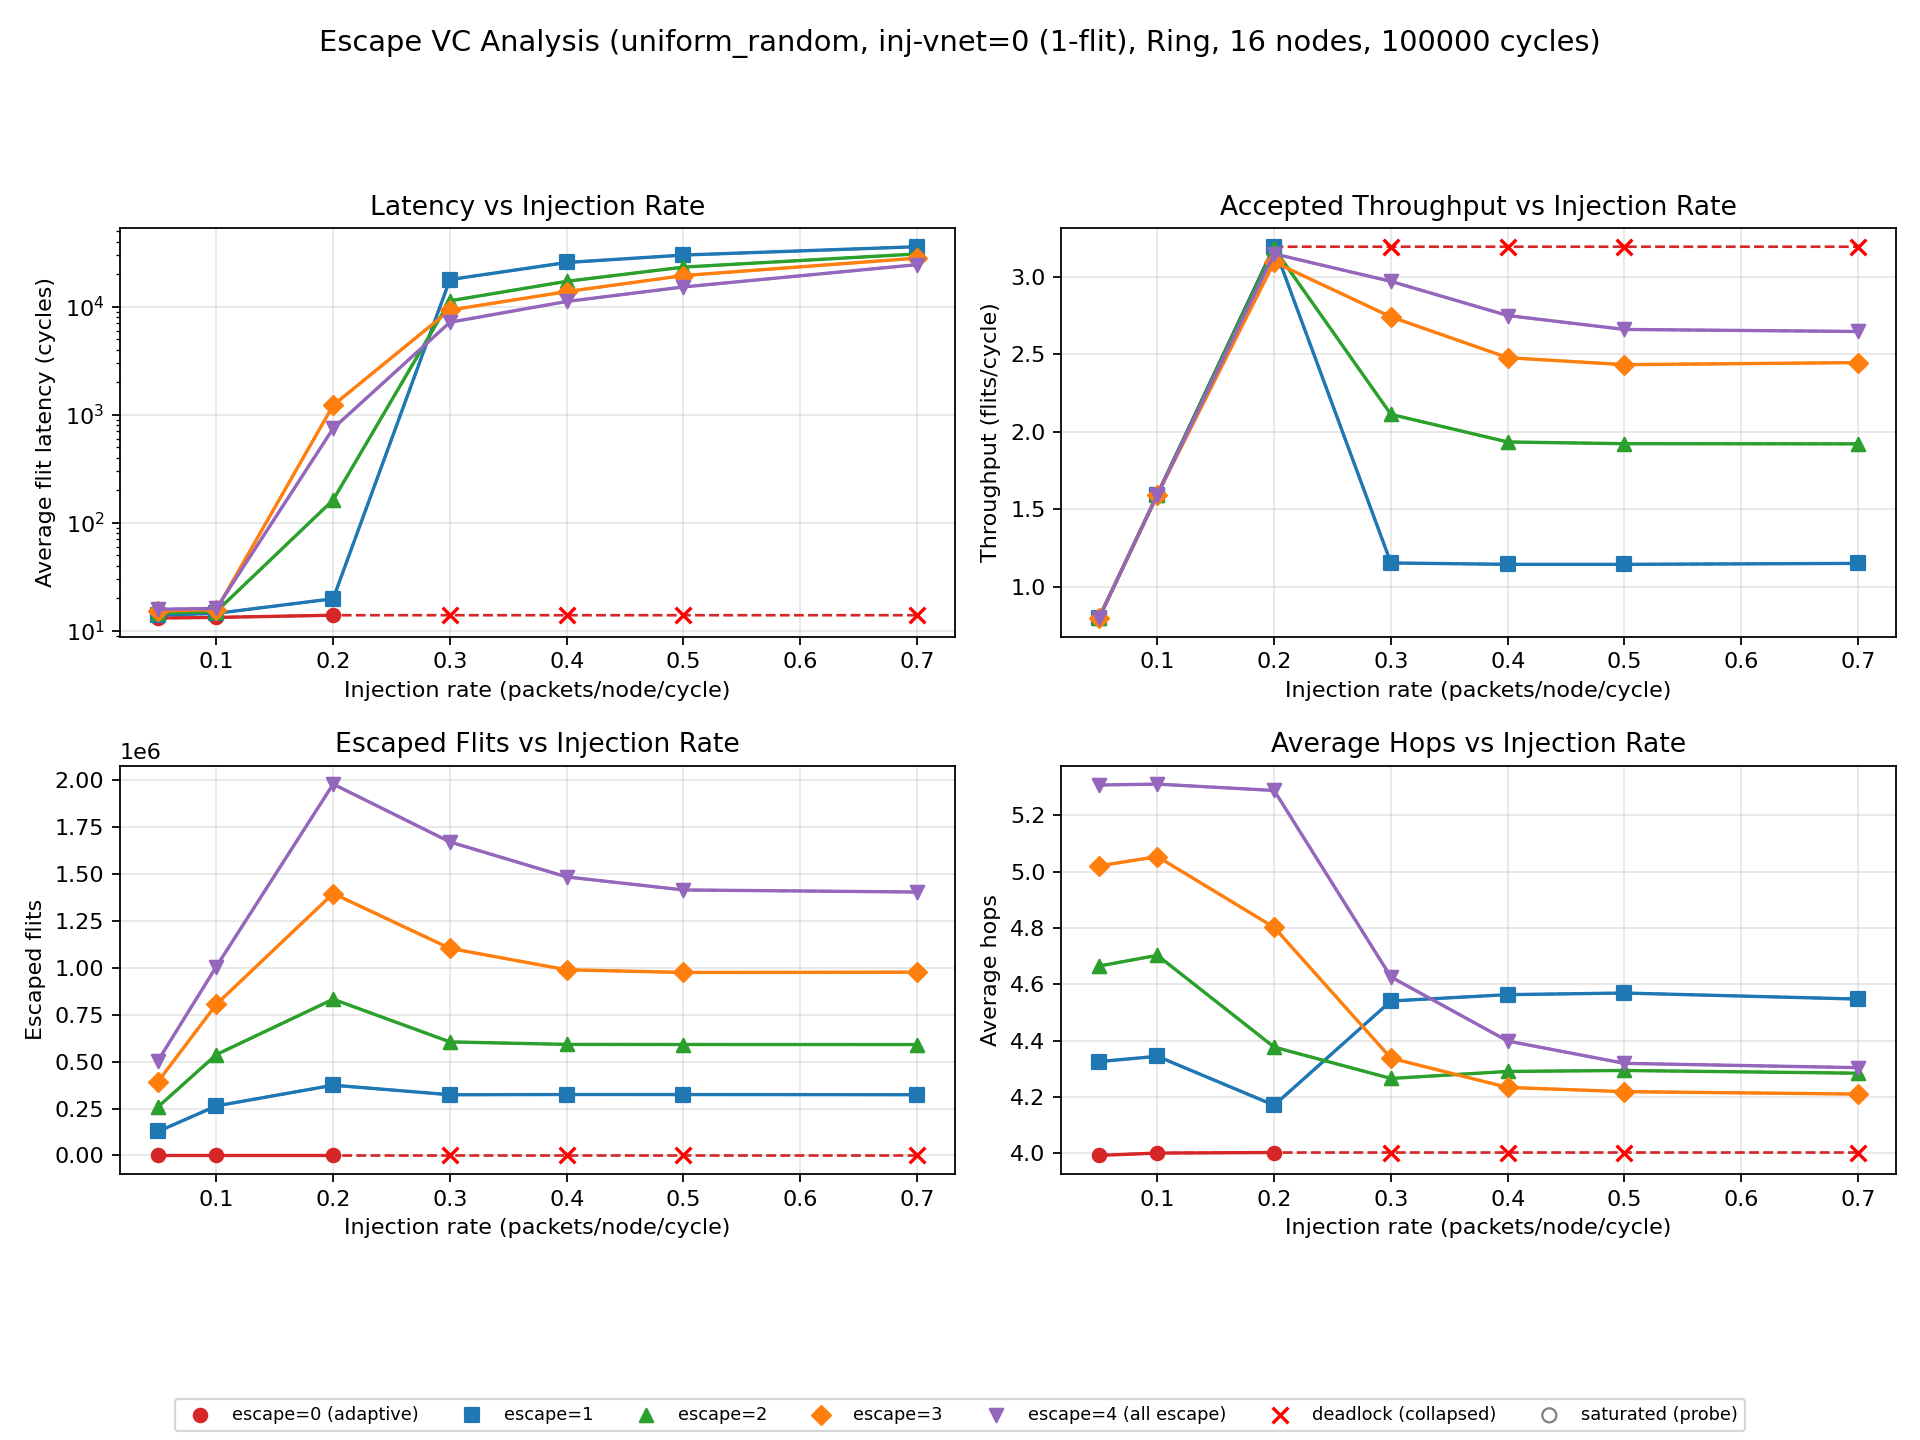
\includegraphics[width=0.7\linewidth]{lab4_escape_injvnet0_analysis.png}
  \caption{Escape-VC sweep ($V=4$, \texttt{uniform\_random},
  \texttt{inj-vnet}=0).  From left to right: flit latency (log scale),
  accepted throughput, escaped-flit count and average hops versus injection
  rate.  Red $\times$ marks deadlocked (collapsed) runs; grey hollow circles
  mark saturated runs measured with a short probe.}
  \label{fig:escape0}
\end{figure}

The escape routing function $R_e$ (\texttt{outportComputeRingEscape}) cuts the
loop at a \emph{dateline} between router $0$ and router $15$ and never lets a
packet wrap around:

\[
  R_e(s,d) = \begin{cases}
    \texttt{Right} & \text{if } d \ge s,\\
    \texttt{Left}  & \text{if } d < s.
  \end{cases}
\]

This turns the ring into a line: every escape packet moves monotonically toward
its destination, so the dependency graph of the escape channels is acyclic and
the escape sub-network is deadlock free.  Because adaptive packets may still
cycle among adaptive VCs, the correctness condition is that any packet is
allowed to ``drop down'' into the escape network; the switch allocator
implements this fallback (Section~\ref{sec:impl:escape}).

\subsection{Design 2: Bubble Flow Control}
\label{sec:arch:bubble}
Bubble flow control attacks deadlock from the buffer side rather than the
routing side.  A ring of single-VC (or few-VC) routers deadlocks only if every
buffer in the cycle becomes occupied.  If we can guarantee that \emph{at least
one buffer (a bubble) is always free} somewhere in each direction of the ring,
the cycle can never close, and any packet can always move into the free slot.
We enforce this with two gates:

\begin{itemize}[itemsep=1pt, topsep=2pt]
  \item \textbf{Injection gate} (in the NI): a node may inject a new packet
        only if the attached router has at least
        $\texttt{BUBBLE\_INJECT\_MIN\_IDLE\_VC}=2$ idle ring input VCs
        \emph{across both directions}.  This keeps injection from filling the
        local router.
  \item \textbf{Ring-entry gate} (in the switch allocator, for $V \ge 2$): a
        head flit may enter a given ring direction only if that direction has
        at least $\texttt{BUBBLE\_ENTER\_MIN\_IDLE\_VC}=2$ idle VCs, which
        keeps $\ge 1$ idle VC (the bubble) per direction at all times.
\end{itemize}

At $V=1$ only the injection gate applies; at $V \ge 2$ the ring-entry gate is
the primary protection.  The thresholds were chosen conservatively (2 idle VCs
rather than 1) so that a transient credit mismatch can never transiently close
the loop.

\section{Implementation}
\label{sec:impl}

All changes are inside \texttt{gem5}'s Garnet network model
(\texttt{src/mem/ruby/network/garnet}) plus the synthetic-traffic configuration
script.  Table~\ref{tab:files} lists the modified/added files.

\begin{table}[H]
  \centering
  \caption{Modified source files.}
  \label{tab:files}
  \small
  \begin{tabular}{@{}ll@{}}
    \toprule
    File & Change \\
    \midrule
    \texttt{configs/example/garnet\_synth\_traffic.py} & add \texttt{--bubble}, \texttt{--escape-vc-per-vnet} \\
    \texttt{configs/topologies/Ring.py} & ring topology (from Lab 3) \\
    \texttt{GarnetNetwork.py / .hh / .cc} & \texttt{escape\_vc\_per\_vnet}, \texttt{bubble} params \& getters \\
    \texttt{CommonTypes.hh} & \texttt{VCClass}, \texttt{RING\_} enum, bubble thresholds \\
    \texttt{RoutingUnit.hh / .cc} & \texttt{outportComputeRing} (adaptive) and \\
                    & \texttt{outportComputeRingEscape} (dateline escape) \\
    \texttt{InputUnit.hh / .cc} & per-VC adaptive/escape output ports \\
    \texttt{VirtualChannel.hh} & \texttt{m\_output\_port\_adaptive / \_escape} fields \\
    \texttt{OutputUnit.hh / .cc} & class-aware \texttt{has\_free\_vc / select\_vc} \\
    \texttt{SwitchAllocator.hh / .cc} & escape fallback, bubble ring-entry gate, \\
                    & \texttt{escaped\_flits} counter \\
    \texttt{Router.hh / .cc} & \texttt{isEscapeVC}, ring-VC accounting, stat \\
    \texttt{NetworkInterface.cc} & bubble injection gate in \texttt{calculateVC} \\
    \bottomrule
  \end{tabular}
\end{table}

\subsection{VC Partitioning and Class-aware Allocation}
\label{sec:impl:escape}
Within a virtual network, VCs are partitioned by index:
escape VCs occupy indices $0 \ldots E-1$ and adaptive VCs occupy $E \ldots V-1$
(\texttt{OutputUnit::vc\_class\_start / vc\_class\_size},
\texttt{Router::isEscapeVC}).  During route computation the \texttt{InputUnit}
computes \emph{both} candidate output ports for each head flit:

\begin{lstlisting}[style=cppstyle, language=C++]
int outport_adaptive = m_router->route_compute(route, inport, dirn, false);
int outport_escape   = m_router->route_compute(route, inport, dirn, true);
grant_outport_adaptive(vc, outport_adaptive);
grant_outport_escape(vc, outport_escape);
\end{lstlisting}

The switch allocator then decides which class to use
(\texttt{SwitchAllocator::arbitrate\_inports}):

\begin{lstlisting}[style=cppstyle, language=C++]
if (escape_in) {                    // packet already in an escape VC
    vc_class = ESCAPE_VC_;
    outport  = outport_escape;
} else if (output(outport_adaptive)->has_free_vc(vnet, ADAPTIVE_VC_)) {
    outport = outport_adaptive;     // stay on the minimal route
} else if (getEscapeVcPerVnet() > 0 &&
           output(outport_escape)->has_free_vc(vnet, ESCAPE_VC_)) {
    vc_class = ESCAPE_VC_;          // fall back: guarantee progress
    outport  = outport_escape;
} else {
    outport = outport_adaptive;     // wait for a future cycle
}
input_unit->grant_outport(invc, outport);
\end{lstlisting}

Once a packet enters an escape VC it \emph{stays} on the escape route for the
rest of its journey (an escape VC only selects \texttt{outport\_escape}), which
is exactly what makes the escape sub-network deadlock free.  The number of
packet heads allocated to escape VCs is counted in
\texttt{SwitchAllocator::m\_escaped\_flits} and reported per router as
\texttt{escaped\_flits}.

\subsection{Bubble Flow Control}
\label{sec:impl:bubble}
The injection gate lives in \texttt{NetworkInterface::calculateVC}:

\begin{lstlisting}[style=cppstyle, language=C++]
if (m_net_ptr->isBubble()) {
    Router *router = m_net_ptr->getRouter(get_router_id(vnet));
    int idle = router->getNumRingVCs()
             - router->getNumActiveRingVCs(vnet);
    if (idle < BUBBLE_INJECT_MIN_IDLE_VC)
        return -1;                  // do not inject yet
}
\end{lstlisting}

\texttt{Router::getNumRingVCs()} counts the input VCs of every non-local input
port (the ring ports), and \texttt{getNumActiveRingVCs(vnet)} counts how many of
them are currently active.  The ring-entry gate lives in
\texttt{SwitchAllocator::send\_allowed} and applies to a head flit that is about
to leave the \texttt{Local} (NI) port into a ring direction:

\begin{lstlisting}[style=cppstyle, language=C++]
if (m_router->get_net_ptr()->isBubble() && !has_outvc &&
    inport_is_local && outport_is_ring &&
    output_unit->getVcsPerVnet() >= 2) {
    if (output_unit->num_idle_vcs(vnet) < BUBBLE_ENTER_MIN_IDLE_VC)
        return false;               // keep >=1 idle VC (bubble)
}
\end{lstlisting}

\subsection{Configuration Interface}
Both mechanisms are exposed through the synthetic-traffic script:

\begin{lstlisting}[style=cppstyle, language=bash]
--bubble                 # enable bubble flow control
--escape-vc-per-vnet=E   # reserve E escape VCs per virtual network
\end{lstlisting}

and propagated to the network object
(\texttt{system.ruby.network.bubble = args.bubble} and
\texttt{system.ruby.network.escape\_vc\_per\_vnet = args.escape\_vc\_per\_vnet}).

\section{Evaluation}
\label{sec:eval}

\subsection{Experimental Setup}
\label{sec:eval:setup}
All experiments use the standalone Garnet build
(\texttt{build/Garnet\_standalone/gem5.opt}) with a 16-node ring, 100\,000
simulation cycles, a 1\,GHz clock, and single-flit packets
(\texttt{--inj-vnet=0}) unless stated otherwise.  Table~\ref{tab:setup}
summarizes the two experiment campaigns.

\begin{table}[H]
  \centering
  \caption{Experimental campaigns.}
  \label{tab:setup}
  \small
  \begin{tabular}{@{}lcc@{}}
    \toprule
    Campaign & \texttt{lab4\_escape.py} & \texttt{lab4\_bubble.py} \\
    \midrule
    Topology & Ring (16) & Ring (16) \\
    Routing & \texttt{routing-algorithm=3} & \texttt{routing-algorithm=3} \\
    VCs per vnet & $V=4$ & $V \in \{1,2,4\}$ \\
    Swept parameter & escape VCs $E \in \{0..4\}$ & bubble on/off, escape on/off \\
    Traffic & \texttt{uniform\_random} & \texttt{uniform\_random}, \\
            & & \texttt{bit\_complement}, \texttt{bit\_reverse} \\
    Inj.\ rate & $0.05 \ldots 0.70$ & $0.01 \ldots 0.70$ \\
    Inj.\ vnet & $-1$ (mixed) and $0$ (1-flit) & $0$ (1-flit) \\
    \bottomrule
  \end{tabular}
\end{table}

Deadlocked runs panic; they are re-run as a short 49\,000-cycle probe and
classified as \emph{collapsed} (true deadlock, probe throughput
$<2.5$ flits/cycle) or \emph{saturated} (congestion only).  In all figures,
red $\times$ marks collapsed runs and grey hollow circles mark saturated probe
points.

\subsection{Escape Virtual Channels}
\label{sec:eval:escape}
Figure~\ref{fig:escape0} (and the mixed-vnet counterpart in
Figure~\ref{fig:escape1}) shows the escape-VC sweep.  Three observations stand
out:

\begin{enumerate}[itemsep=1pt, topsep=2pt]
  \item \textbf{Deadlock elimination.} With $E=0$ (pure adaptive) the network
        \emph{collapses} at injection rates $\ge 0.3$ (inj-vnet 0) or
        intermittently from $0.2$ onward (mixed vnets).  Any $E \ge 1$ removes
        every collapsed point: deadlock is fully eliminated, exactly as the
        theory predicts.
  \item \textbf{Escape channels are a bottleneck.} At high load the accepted
        throughput of $E=1$ ($\approx 1.15$ flits/cycle) is much lower than
        that of $E=4$ ($\approx 2.7$ flits/cycle).  With only one escape VC
        per router, packets that fall back to the escape route serialize onto
        a single channel and take the (non-minimal) dateline path, inflating
        both latency and hop count.
  \item \textbf{Path-length penalty.} The average hop count grows with $E$
        (from $\approx 4.0$ adaptive to $\approx 5.3$ for all-escape routing)
        because the dateline route is no longer always minimal.
  \end{enumerate}

\begin{figure}[H]
  \centering
  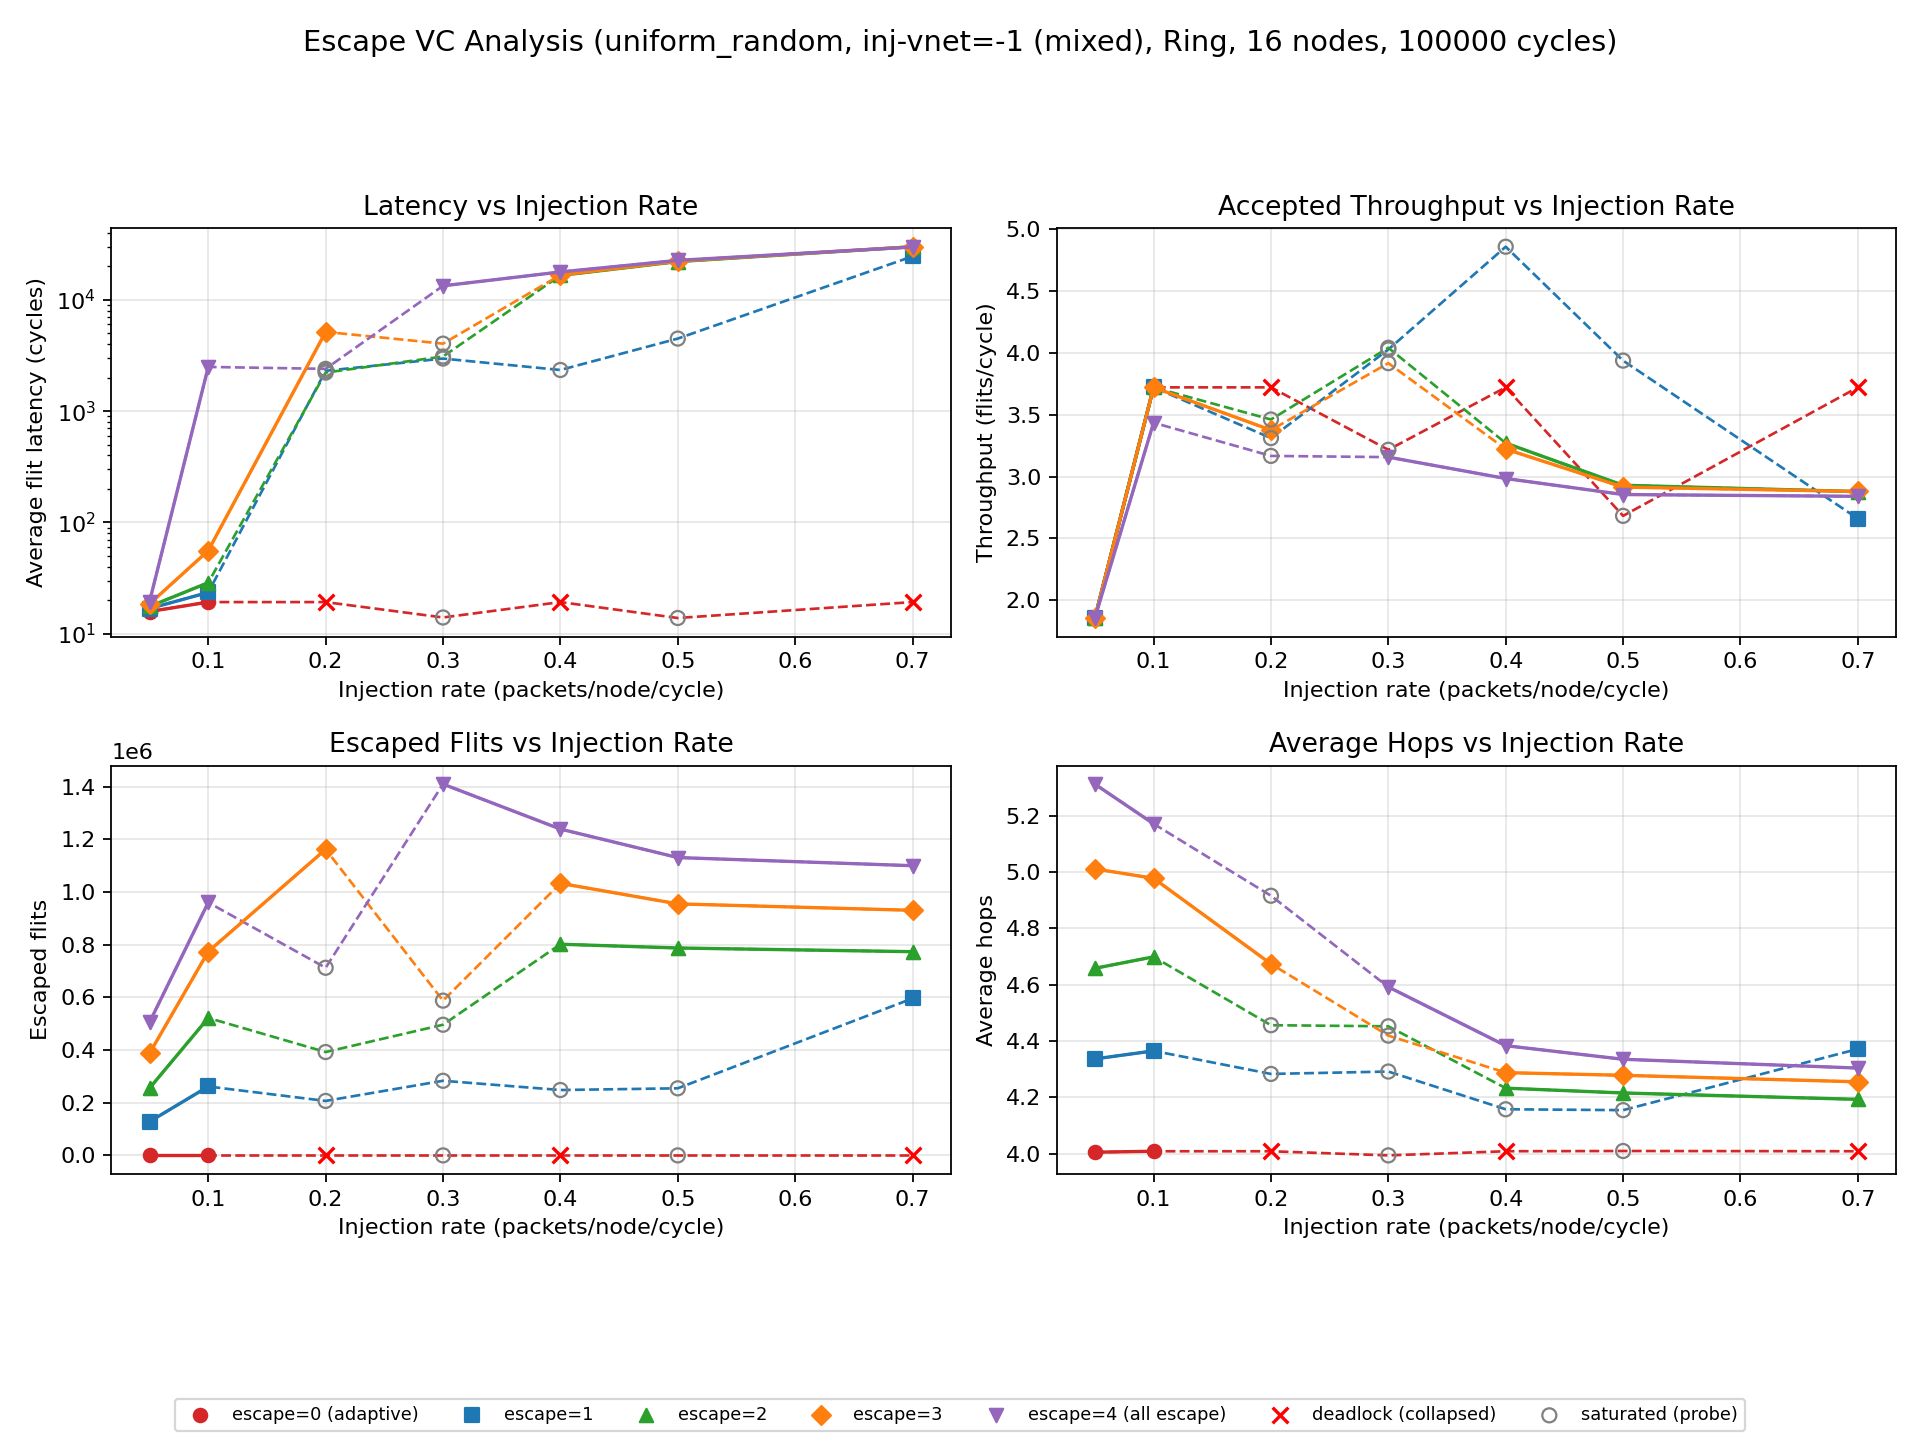
\includegraphics[width=0.7\linewidth]{lab4_escape_injvnet-1_analysis.png}
  \caption{Escape-VC sweep for mixed virtual networks
  (\texttt{inj-vnet=-1}, 1-flit and 5-flit packets mixed).}
  \label{fig:escape1}
\end{figure}

\subsection{Bubble Flow Control}
\label{sec:eval:bubble}
Figures~\ref{fig:bubble_vc1}--\ref{fig:bubble_vc4} compare, for each VC count,
the naive baseline, the bubble configuration and (where applicable) the escape
configuration under \texttt{uniform\_random} traffic.

\begin{figure}[H]
  \centering
  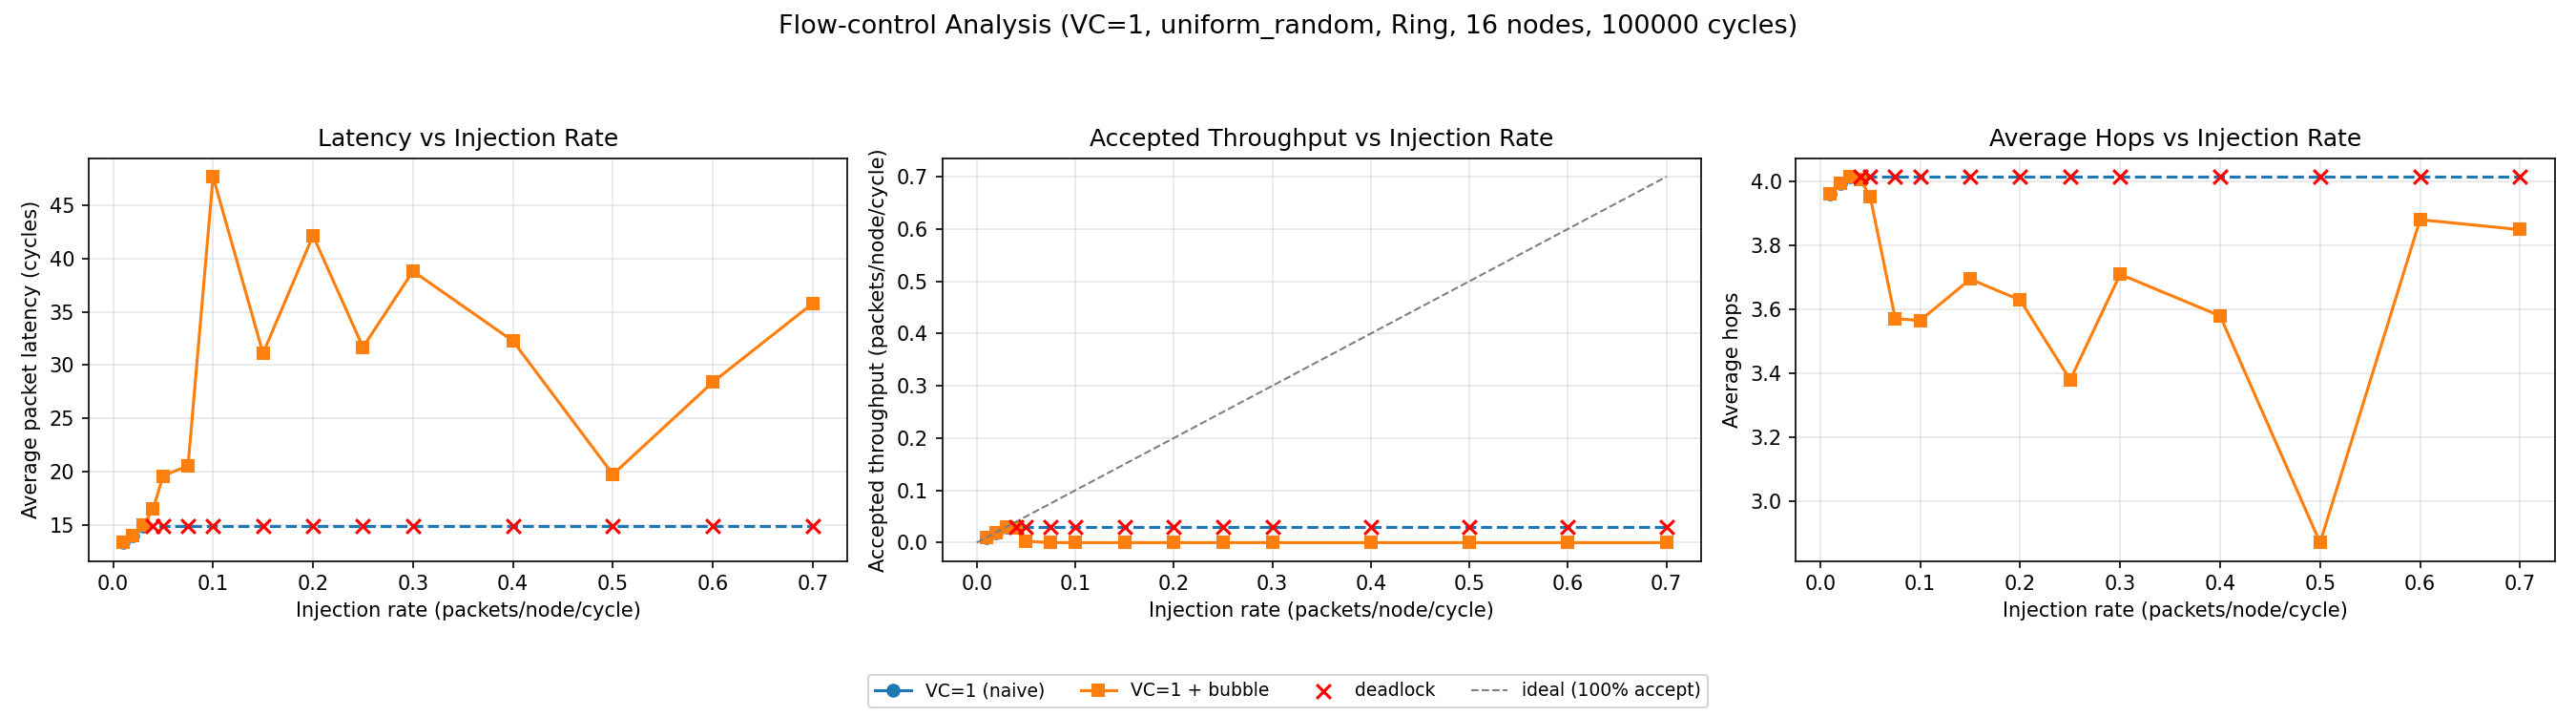
\includegraphics[width=0.78\linewidth]{lab4_bubble_uniform_random_vc1_analysis.png}
  \caption{Bubble analysis at $V=1$ (\texttt{uniform\_random}).}
  \label{fig:bubble_vc1}
\end{figure}

\begin{figure}[H]
  \centering
  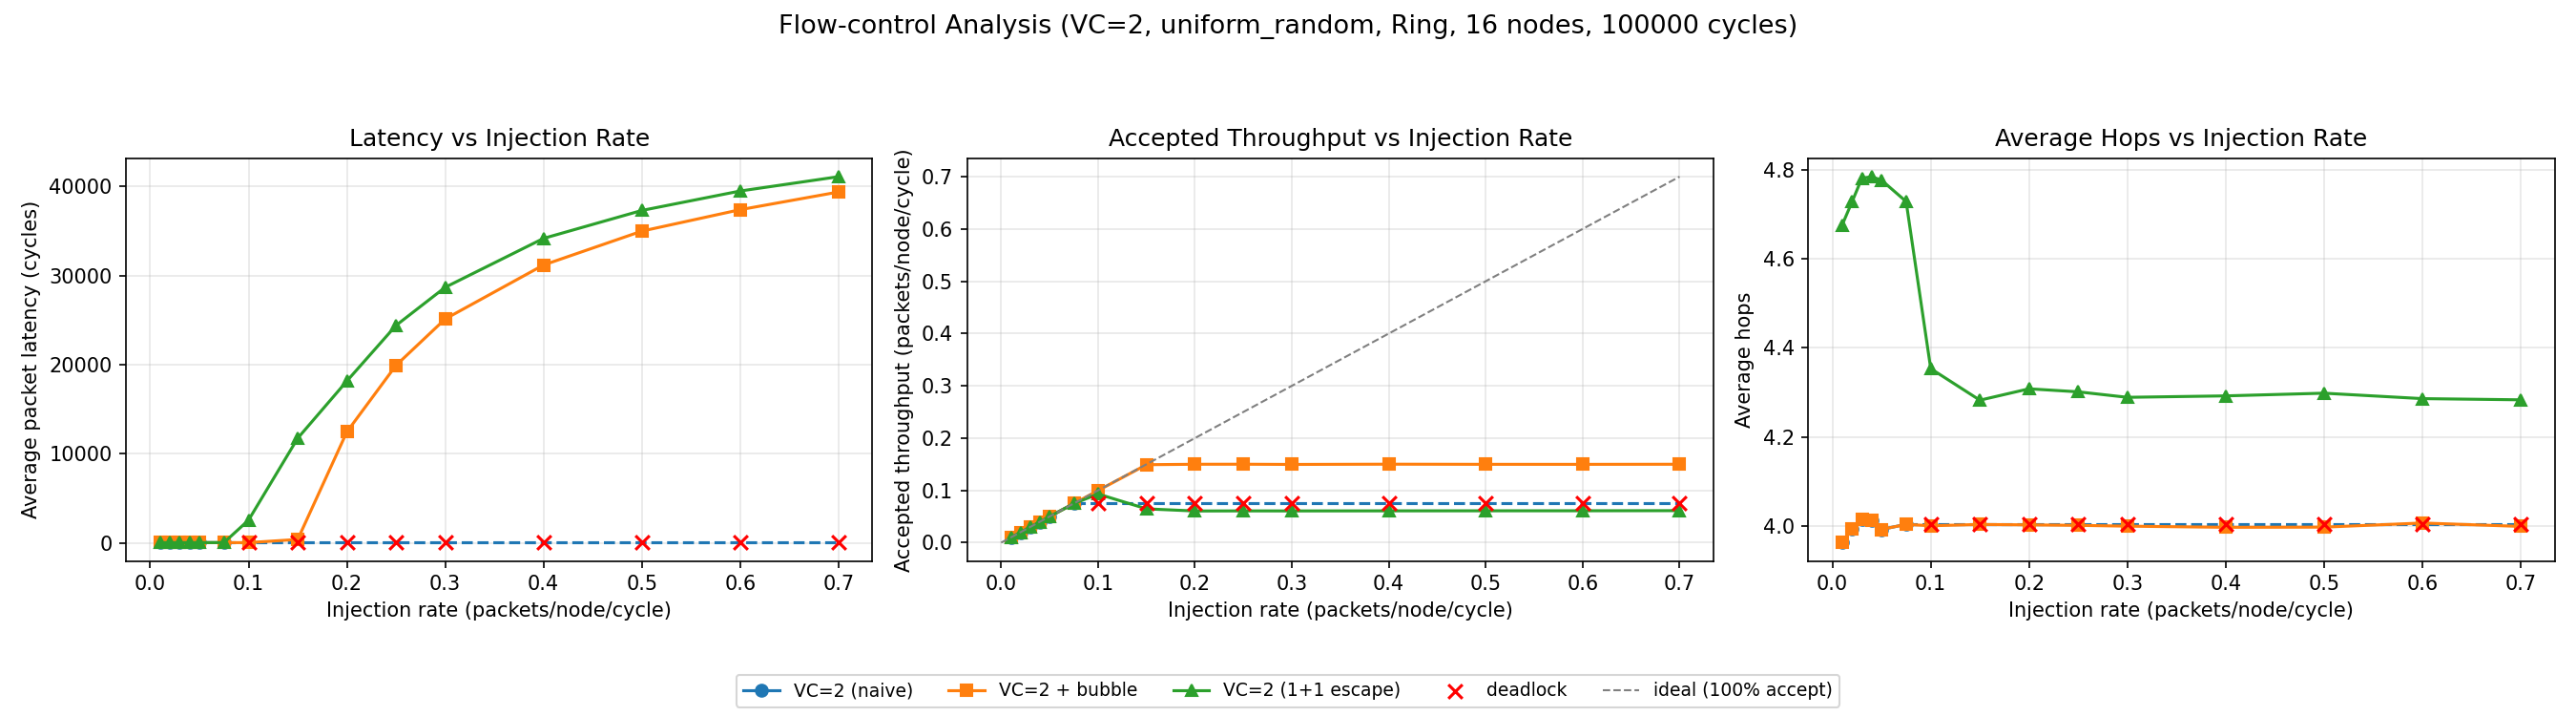
\includegraphics[width=0.78\linewidth]{lab4_bubble_uniform_random_vc2_analysis.png}
  \caption{Bubble analysis at $V=2$ (\texttt{uniform\_random}).}
  \label{fig:bubble_vc2}
\end{figure}

\begin{figure}[H]
  \centering
  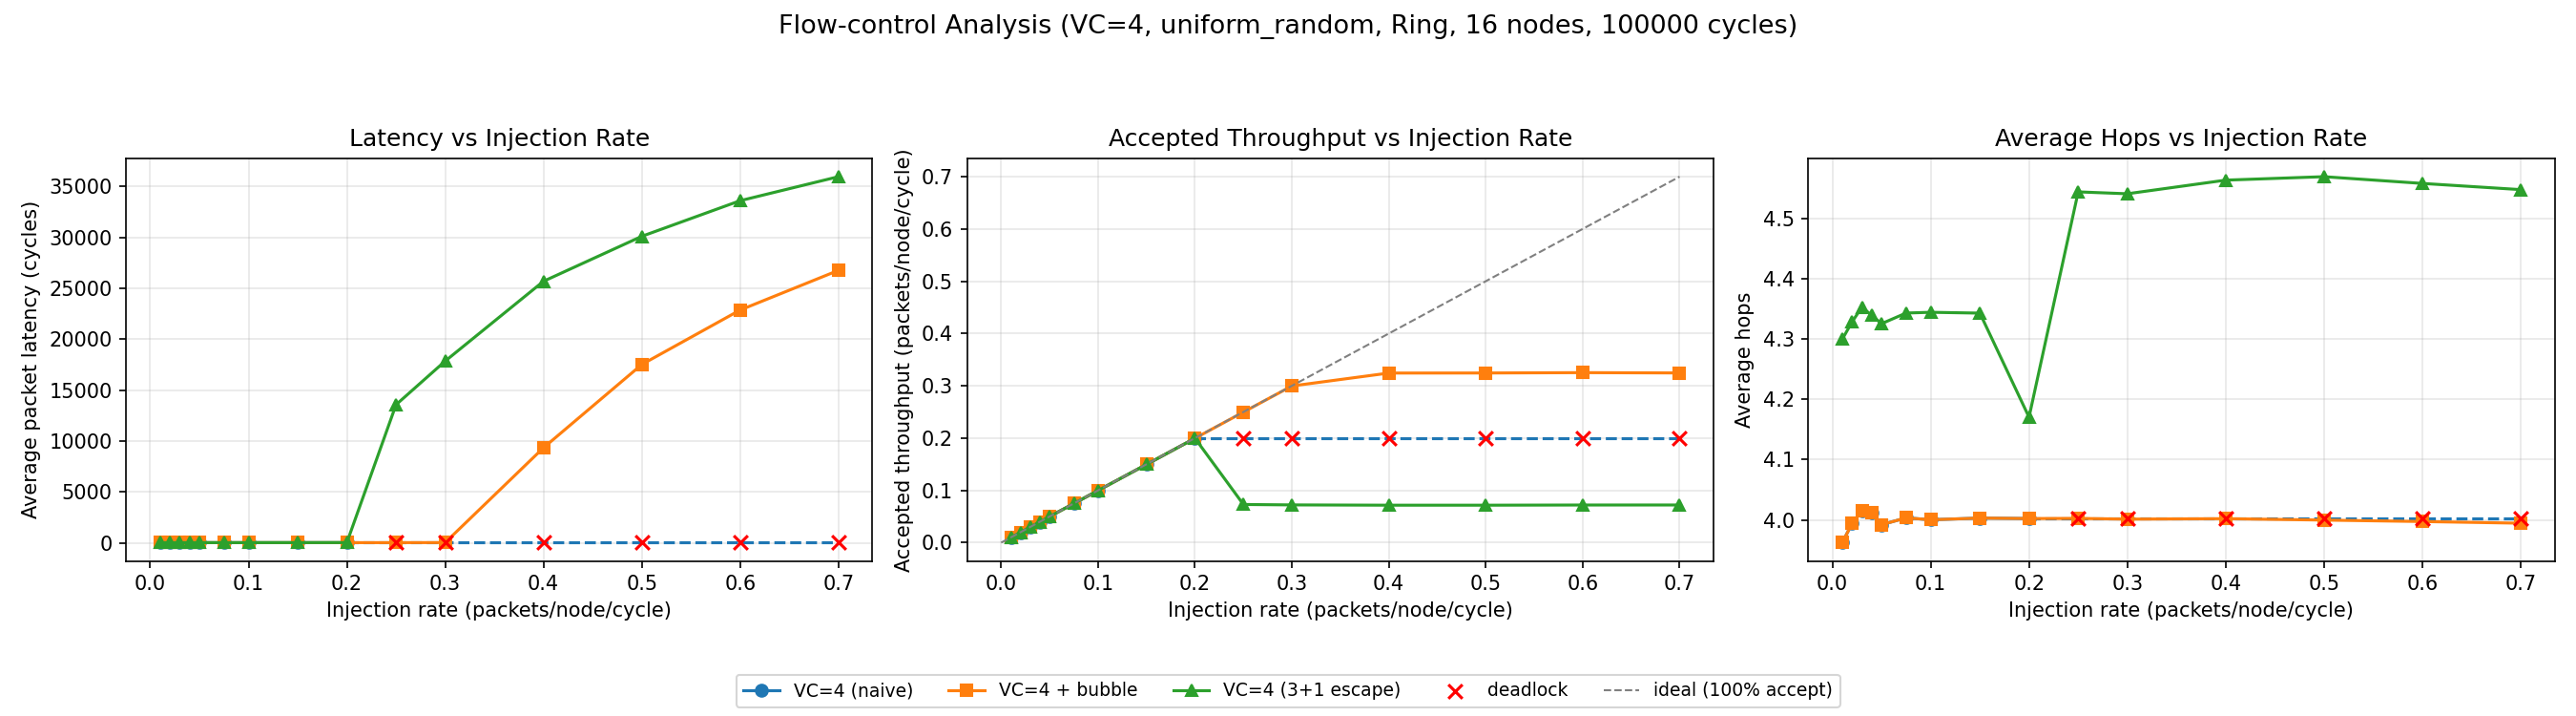
\includegraphics[width=0.78\linewidth]{lab4_bubble_uniform_random_vc4_analysis.png}
  \caption{Bubble analysis at $V=4$ (\texttt{uniform\_random}).}
  \label{fig:bubble_vc4}
\end{figure}

The key findings are:

\begin{enumerate}[itemsep=1pt, topsep=2pt]
  \item \textbf{Naive baselines deadlock.} At $V=1$ the naive network collapses
        by rate $0.075$; at $V=2$ by $0.1$--$0.15$; even at $V=4$ it collapses
        beyond saturation ($0.25$--$0.3$ for \texttt{bit\_complement}).  More
        VCs only postpone the onset of the cyclic wait; they do not remove the
        cycle itself.
  \item \textbf{Bubble prevents deadlock, but over-throttles $V=1$.} With a
        single VC the bubble injection gate is too restrictive: from rate
        $0.05$ onward only a handful of flits are delivered and the network
        effectively starves.  A single VC has no slack, so keeping a free VC
        means keeping $\approx$ half the ring idle.
  \item \textbf{Bubble wins at $V \ge 2$.} At $V=2$ and $V=4$ bubble flow
        control removes all collapsed points and sustains the highest
        saturated throughput (e.g., $\approx 0.15$ flits/node/cycle at $V=2$
        and $\approx 0.32$ at $V=4$ for \texttt{uniform\_random}), while the
        escape configurations saturate lower ($\approx 0.06$ at $V=2$ with
        $1+1$ and $\approx 0.07$ at $V=4$ with $3+1$).  The reason is that
        bubble keeps \emph{minimal} routing, whereas escape VCs divert a
        significant fraction of packets onto the longer dateline route.
  \item \textbf{Traffic sensitivity.} \texttt{bit\_reverse} is the most
        benign pattern (it is an involution that pairs sources and
        destinations), so all mechanisms survive to higher rates; adversarial
        patterns such as \texttt{bit\_complement} expose deadlock earliest.
  \end{enumerate}

\subsection{Summary Comparison}
\label{sec:eval:compare}
Table~\ref{tab:compare} condenses the qualitative comparison of the two
techniques.

\begin{table}[H]
  \centering
  \caption{Qualitative comparison of the two flow-control techniques.}
  \label{tab:compare}
  \small
  \begin{tabular}{@{}lcc@{}}
    \toprule
    Property & Escape VC & Bubble \\
    \midrule
    Deadlock freedom & guaranteed (dateline) & guaranteed (free buffer) \\
    Routing & becomes non-minimal & stays minimal \\
    Extra hardware & extra VC buffers & none (throttling only) \\
    Saturation throughput & lower (escape bottleneck) & higher ($V\ge2$) \\
    Behaviour at $V=1$ & works & starves (over-throttled) \\
    Implementation cost & moderate & small \\
    \bottomrule
  \end{tabular}
\end{table}

The two techniques are therefore complementary: escape VCs are the robust
general mechanism (they work at any VC count and scale to arbitrary topologies
via turn-model/dateline routing), while bubble flow control is cheaper and
higher-performing but only sensible when the router has $\ge 2$ VCs of slack.

\section{Division of Labor}
\label{sec:labor}

\begin{itemize}[itemsep=2pt, topsep=2pt]
  \item \textbf{Member A (name, ID):} ring topology and adaptive ring routing
        baseline; escape-VC routing function and VC partitioning;
        \texttt{lab4\_escape.py} experiments and analysis.
  \item \textbf{Member B (name, ID):} bubble flow-control gates; class-aware
        VC allocation and \texttt{escaped\_flits} statistics;
        \texttt{lab4\_bubble.py} experiments and analysis.
  \item \textbf{Both:} report writing and presentation.
\end{itemize}

\section{Conclusion}
\label{sec:conclusion}

We implemented and evaluated two flow-control techniques --- escape virtual
channels and bubble flow control --- that make the adaptive shortest-path
routing of a 16-node ring deadlock free.  Escape VCs provably eliminate
deadlock by routing through a dateline-cut escape network, at the cost of
non-minimal paths and a bottleneck at the escape channels.  Bubble flow
control prevents deadlock with no extra buffers by keeping a free VC in every
ring direction, and achieves the highest saturation throughput for routers
with at least two VCs, but it over-throttles a single-VC network.  The
evaluation confirms the theory on real synthetic traffic and quantifies the
throughput/latency trade-off between the two approaches, providing a clear
basis for choosing a flow-control strategy for ring-based networks-on-chip.

\bibliographystyle{plain}
\begin{thebibliography}{9}

\bibitem{dally1987deadlock}
W.~J. Dally and C.~L. Seitz,
``Deadlock-free message routing in multiprocessor interconnection networks,''
\emph{IEEE Transactions on Computers}, vol.~C-36, no.~5, pp.~547--553, 1987.

\bibitem{duato1993new}
J.~Duato,
``A new theory of deadlock-free adaptive routing in wormhole networks,''
\emph{IEEE Transactions on Parallel and Distributed Systems}, vol.~4,
no.~12, pp.~1320--1331, 1993.

\bibitem{puente1999bubble}
V.~Puente, R.~Beivide, J.~A. Gregorio, J.~M. Prellezo, J.~Duato, and C.~Izu,
``Adaptive bubble router: a design to improve performance in torus networks,''
in \emph{Proc.\ Int.\ Conf.\ on Parallel Processing (ICPP)}, 1999.

\bibitem{gem5}
N.~Binkert et al., ``The gem5 simulator,'' \emph{ACM SIGARCH Computer
Architecture News}, vol.~39, no.~2, pp.~1--7, 2011.

\end{thebibliography}

\end{document}
